\glsresetall
\section{Concept}
\label{sec:concept}
Chapter~\ref{sec:preliminaries} has laid the theoretical foundations needed to describe the concept of this thesis. In the first section, the environment is defined with a focus on three aspects: The state space \statespace, which is defined by a hybrid input representation using numerical and image input. Then the reward function is described, before the action space \actionspace\ is defined. Next is a derivation of the $\tanh$-squashed Normal distribution, which is motivated by the need to constrain actions within the physical boundaries of a vehicle. In the following section, an objective function for multi-agent scenarios is obtained by extending a formulation of the AlphaZero loss for continuous action spaces. How a Transformer-based network architecture can be used to handle scenarios with a flexible number of agents comes next. The penultimate section describes a guided \gls{mcts} procedure, where rollouts are truncated by network evaluations. Finishing up the chapter is the concept of a training algorithm for the system.

\subsection{Environment}\label{ssec:environment}
Section~\ref{sssec:dec_mdp} has introduced the theoretical framework of a \gls{dmdp} as a tuple \dmdptuple. Now it is time to elaborate further on how some of its components are implemented concretely. Of particular interest are the state space \statespace, the action space \actionspace\ and the reward function $\mathcal R (\cdot)$. Section~\ref{sssec:input_representation} details a hybrid input representation consisting of a local visual map of an agent together with numerical information about all other vehicles in a scenario. It can be processed efficiently by a neural network. This characterizes the state space \statespace. Next is the definition of the reward function $\mathcal R (\cdot)$, before a brief description of the action space \actionspace\ follows. How the chosen actions are mapped to vehicle trajectories finishes the chapter. 

\subsubsection{Input Representation}\label{sssec:input_representation}
In general, a state \state\ in the \gls{dmdp} is given by a scenario. It in turn is defined as a road with multiple lanes, a set of active agents executing actions and optionally a set of stationary vehicles (obstacles) on the road. Surrounding the road is non-drivable area. The number of lanes, active agents and obstacles as well as their position is flexible and different for each scenario.
\begin{figure}[!h]
\centering
\includesvg[width=\textwidth]{scenarios/sc10}
\caption[Scenario example]{Example of a cooperative driving scenario where two agents have to avoid a crash while driving through a narrow bottleneck.}
\label{fig:scenario_example}
\end{figure}
Figure~\ref{fig:scenario_example} shows the map for such a scenario, where two agents have to drive through a bottleneck. In order to avoid a crash, one vehicle will have to slow down and the other must accelerate while both merge into the center. This maneuver requires cooperation between both agents \cite{kurzerDecentralizedCooperativePlanning2018}.

How can such a scenario be encoded in a way that is both efficient to process for a neural network as well as close to real-world autonomous driving? To answer this question, a hybrid input representation consisting of both a visual map and a set of numerical inputs is chosen \cite{bacchianiMicroscopicTrafficSimulation2019, kurzerAcceleratingCooperativePlanning2020}. The map is a top down view of the agent's region of interest in the scenario that is defined by its sensor range. It covers an area of $64m$ forwards and backwards as well as $6.4m$ to each side from the center of a vehicle's back axle. The total viewable area is thus $128m \times 12.8m$. This is encoded into a two channel image of $2 \times 32 \times 64$ pixels, where the first channel is an agent map that solely encodes the active agents in the scenario. 
\begin{figure}[!t]
	\centering
	\captionsetup{justification=centering}
    \scalebox{0.6}{\input{images/agent_view.pdf_tex}}
	\caption[Agent view example]{Example of an agent's view from scenario 08 (Figure~\ref{fig:scenario_example}). Active agents are depicted in yellow, whereas obstacles (stationary vehicles) are represented as non-drivable area on the lane. The lanes are colored in different shades of purple.}
\label{fig:agent_view}
\end{figure}
The second channel represents lanes, obstacles and non-drivable area. Obstacles are using the same numerical values as non-drivable area. This allows for a more efficient representation using only two channels instead of three. Since an agent receives the same reward for crashing into an obstacle as it does for driving off the road, no distortion between its perception and its immediate reward occurs. This is discussed further in Section~\ref{sssec:scenario_rewards} (also see Appendix~\ref{app:reward_params}). Figure~\ref{fig:agent_view} shows an example of an agent's view in scenario 08.

Lastly, it is important to note that the resolution of the visual map is coarse due to performance constraints\footnote{Profiling the executable reveals that the program spends around $9.5 \%$ of its runtime generating the maps. This can quickly jump to over $40 \%$ for higher resolutions.}. Particularly for longitudinal maneuvers, $2$ meters per pixel might not seem granular enough. A consideration however is that lateral maneuvers usually require more precision, for instance when avoiding an obstacle. This is still allowed by  a finer lateral resolution of $0.4$ meters per pixel.

Visual input representations have the advantage that they are flexible and environment-agnostic. As described above, there is however a trade-off between representational capacity and computational efficiency. Numerical inputs on the other hand are less computationally expensive and allow for detailed information but need to be tailored to a specific task. Since the goal of this thesis is learning cooperative driving behavior, it is sensible to additionally encode agent information numerically to foster interaction. The state of a single agent $i$ at time step $t$ is composed of a static state vector $\mathbf n_i^{\text{static}}$ and dynamic state vectors $\mathbf n_i^{\text{dynamic}} (t)$ \cite{kurzerAcceleratingCooperativePlanning2020}. The static component of the state refers to agent information that does not change over the course of a scenario whereas the dynamic component changes with each time step $t$. Concatenation of the current dynamic state vector with the past seven dynamic state vectors and the static state vector yields the full numerical state of an agent. It is represented in  Equation~\ref{eq:simple_numerical_rep}, where $\oplus$ represents the concatenation operation. While combining past information into a Markovian state might seem redundant at first, it produces little computational overhead due to the efficiency with which numerical values are processed. At the same time it ensures that agents have access to all needed information \cite{kurzerAcceleratingCooperativePlanning2020}. Similar techniques like "\emph{frame-stacking}", where the past $m$ images are combined into a single stacked image, are also common in other \gls{rl} applications \cite{mnihHumanlevelControlDeep2015}.
\begin{align}\label{eq:simple_numerical_rep}
    \mathbf n_i^{\text{dynamic}} (t) & = \big( x_i (t), \, y_i (t), \, \dot x_i (t), \, \dot y_i (t), \, \ddot x_i (t), \, \ddot y_i (t), \, \phi_i (t) \big) \nonumber \\
    \mathbf n_i^{\text{static}} & = \big( \dot x_i^{\text{desire}}, \, l_i^{\text{desire}}, v_i^{\text{width}}, v_i^{\text{length}} \big) \nonumber \\ 
    \mathbf n_i (t) & = \mathbf n_i^{\text{dynamic}} (t-7) \oplus \mathbf n_i^{\text{dynamic}} (t-6) \oplus \ldots \oplus \mathbf n_i^{\text{dynamic}} (t) \oplus \mathbf n_i^{\text{static}}~.
\end{align}
More concretely:
\begin{itemize}
    \item $(x_i(t), \, y_i(t))$ is the normalized relative position of agent $i$.
    \item $(\dot x_i(t), \, \dot y_i(t))$ is the normalized relative velocity of agent $i$ in lateral and longitudinal direction.
    \item $(\ddot x_i (t), \, \ddot y_i (t))$ is the normalized relative acceleration of agent $i$ in each direction.
    \item $\phi_i (t)$ is agent $i$'s normalized relative heading in radian.
    \item $\dot x_i^{\text{desire}}$ is the desired velocity of agent $i$ in longitudinal direction.
    \item $l_i^{\text{desire}}$ is the desired lane of agent $i$.
    \item $(v_i^{\text{width}}, v_i^{\text{length}})$ are the vehicle dimensions of agent $i$.
\end{itemize}
It is important to highlight that dynamic state information is given \emph{relative to the ego agent}. That is, relative to the agent currently making the decision. During each scenario run all agents sense each other with limited sensor precision outside of the $128m \times 12.8m$ region of interest. The limited precision is modeled by bounding relative values on the interval $[-1, 1]$. To give an example, suppose $x_1=10$ is the longitudinal position of agent one while $x_2=138$ is the longitudinal position of agent two. Then the relative longitudinal position of agent two with respect to agent one is $x_2^{\text{rel}} = 128$. Normalizing by the maximum frontal sensor range of agent one yields $x_2^{\text{rel, norm}} = 128/64 = 2$. However, since agent two has been outside of agent one's sensor range, $x_2^{\text{rel, norm}}$ is capped at $1$. This reflects the limited precision of sensors over longer ranges. Intuitively, agent one can sense another vehicle approaching but its distance is too far to take exact measurements.

The full numerical state of an agent $i$ within a scenario is given as the matrix produced by stacking the numerical states $\mathbf n_i (t)$ of all agents $\Upsilon$ within the scenario:
\begin{gather}\label{eq:full_numerical_rep}
   \mathbf s_i^{\text{num}} (t) =  \begin{pmatrix}
    \mathbf n_0 (t)\\
    \mathbf n_1 (t)\\
    \vdots\\
    \mathbf n_\Upsilon (t)
    \end{pmatrix}~.
\end{gather}
It is worth repeating that all numerical states in $\mathbf s_i^{\text{num}} (t)$ are relative to the current agent $i$. Now that the state space \statespace\ of the environment is defined, the next section can introduce the reward function $\mathcal R$.

\subsubsection{Reward function}\label{sssec:scenario_rewards}
The reward function of an \gls{rl} environment is key in eliciting the desired behavior from an agent. Actions that are desired should be reinforced while actions leading to undesired or even harmful behavior should be punished. Ideally, the reinforcement comes immediately after a specific action, making the reward function \emph{dense}. The opposite of dense rewards are \emph{sparse} rewards. An example of a sparse reward environment is the game of chess: Here an agent only receives a positive or negative reward upon completion of the game but not for any intermediate actions. Therefore the following paragraphs specify a dense reward function composed of three parts (see Equation~\ref{eq:reward_components}) \cite{kurzerDecentralizedCooperativePlanning2018}:
\begin{enumerate}
    \item A component which punishes actions that are too jerky, thereby encouraging smooth driving maneuvers.
    \item A term that rewards an agent depending on its distance to a desired target state , which is specified by a target velocity $\dot x_i^{\text{desire}}$ and a target lane $l_i^{\text{desire}}$.
    \item A validity component punishing actions that lead to either collisions or driving off the road.
\end{enumerate}
The components outlined above define the ego reward for each agent. It is a sum of three elements \cite{kurzerDecentralizedCooperativePlanning2018}:
\begin{gather}\label{eq:reward_components}
    r_i = r_i^{\text{action}} + r_i^{\text{state}} + r_i^{\text{valid}}~.
\end{gather}
Its first term is the \emph{action reward} $r_i^{\text{action}}$. It is always negative and can be interpreted as the cost of performing a driving maneuver between two time steps $t_0$ and $t_1$ \cite{kurzerDecentralizedCooperativePlanning2018}. The action reward consists of the following components
\begin{gather}\label{eq:reward_action}
    r_i^{\text{action}} = w_{LC} ( l_i (t_1) - l_i (t_0) )^2 + w_{AX} \int_{t_0}^{t_1} (\ddot x_i(t))^2 dt + w_{AY} \int_{t_0}^{t_1} (\ddot y_i(t))^2 dt + w_{IA}~.
\end{gather}
The first term $( l_i (t_1) - l_i (t_0) )^2$ punishes lane changes while the second $\int_{t_0}^{t_1} (\ddot x_i(t))^2 dt$ and third term $\int_{t_0}^{t_1} (\ddot y_i(t))^2 dt$ aim at minimizing the acceleration in longitudinal and lateral direction. The relative importance of each component can be adjusted via the weights $w_{LC}, w_{AX}$ and $w_{AY}$. $w_{IA}$ is a constant that is added if the generated action is invalid, for instance when the vehicle's steering angle is past its maximum or the agent exceeds the maximum speed limit \cite{kurzerDecentralizedCooperativePlanning2018}.

Next is the \emph{state reward} $r_i^{\text{state}}$ aimed at minimizing the distance between the current state and a desired target state of the agent \cite{kurzerDecentralizedCooperativePlanning2018}:
\begin{align}\label{eq:reward_state}
    r_i^{\text{state}} = {} &  \underbrace{2 w_{VD} \cdot \exp \big(-0.00745 \cdot (\dot x_i^{\text{desire}} - \dot x_i(t))^2 \big) - w_{VD}}_\text{Velocity component} \nonumber \\
    & +  \underbrace{w_{LD} - w_{LCD} \big|l_i (t) - l_i^{\text{desire}}}_\text{Lane deviation component} \big|  \nonumber \\
    & + \underbrace{w_{LCD} \cdot \exp \Big(-5.0 \frac{c_i^l (t) -y_i(t)}{2 \cdot W_l} \Big)}_\text{Lane center deviation component}~.
\end{align}
Subscripts for the time step $t$ in Equation~\ref{eq:reward_state} are dropped as quantities are only evaluated at the current step $t$. The weight $w_{VD}$ is used to scale the velocity deviation term. It is defined using an exponential function $\exp \big(-0.00745 \cdot (\dot x_i^{\text{desire}} - \dot x_i(t))^2 \big)$ with a quadratic exponent \cite{kurzerDecentralizedCooperativePlanning2018}. If the agent's current velocity $\dot x_i(t)$ reaches its desired velocity $\dot x_i^{\text{desire}}$, the whole exponential reduces to the factor $1$, thus maximizing the velocity deviation reward as $w_{VD}$.

The lane deviation component is composed of a positive weight $w_{LD}$, from which the weighted absolute lane deviation $w_{LCD} \big|l_i (t) - l_i^{\text{desire}} \big|$ is subtracted. Here $w_{LCD}$ is the lane center deviation weight. If for instance the agent's target lane is $l_i^{\text{desire}} = 3$ and its current lane $l_i (t) = 1$, then $w_{LCD} \cdot 2$ is subtracted \cite{kurzerDecentralizedCooperativePlanning2018}.

Lastly, the deviation from the lane center is rewarded using an exponential term similar to the velocity deviation term. It is subsequently weighted by the lane center deviation weight $w_{LCD}$. If the vehicle is exactly on the center line of the lane it is currently driving on (denoted as $c_i^l (t)$), the denominator reduces to $0$ and the whole center deviation reward becomes $ w_{LCD}$. The term in the numerator is defined as two times the lane width $W_l$ in the current scenario\footnote{Lanes are assumed to have equal width in all scenarios.} \cite{kurzerDecentralizedCooperativePlanning2018}.

Combining everything above, the maximum state reward achievable is the sum of the three weights $w_{VD} + w_{LD} + w_{LCD}$. This is accomplished if the agent drives exactly center on its target lane and with the desired velocity. The exact values of the weights $w_{VD}, w_{LD}$ and $w_{LCD}$ may be adjusted individually for each scenario.

The last component of the reward function in Equation~\ref{eq:reward_components} is the \emph{validation reward} \cite{kurzerDecentralizedCooperativePlanning2018}:
\begin{align}
    r_i^{\text{valid}} = \begin{cases} w_{IS}, & \text{if invalid state} \\ w_{C}, & \text{if collision} \\ 0, & \text{else} \end{cases}~.
\end{align}
$w_{IS}$ is a constant added if the action leads to an invalid state. That is, if the vehicle leaves the road and is in non-drivable area. The reward $w_{C}$ is given if the action results in a collision with another vehicle or obstacle. When neither of the above occurs, the chosen action is deemed valid and nothing is added. Usually the weights for invalid states and collisions are set to large negative constants (e.g. $w_{IS} = w_{C} = -1000$) as both states are highly undesirable \cite{kurzerDecentralizedCooperativePlanning2018}.

The three components described above fully define the ego reward for an agent. While the validation reward is straightforward, there is a push-pull dynamic between the action reward and the state reward: On one hand, an agent wants to reach its target state as quickly as possible through the state reward. One the other hand, abrupt maneuvers are punished more severely by the action reward. Together they form a balance in which an agent tries to achieve its goal state quickly but also economically \cite{kurzerDecentralizedCooperativePlanning2018}.

To achieve cooperation and fully specify the reward function $\mathcal R$ of the environment, one last component is missing. It is the cooperative reward. Given a cooperation factor $\lambda_i$, the cooperative reward $r^{\text{coop}}_i$ of an agent $i$ is defined as \cite{kurzerDecentralizedCooperativePlanning2018}:
\begin{gather}\label{eq:coop_reward}
    r^{\text{coop}}_i = r_i + \lambda_i \sum_{j=0, j \neq i}^{\Upsilon} r_j
\end{gather}
Here $\sum_{j=0, j \neq i}^{\Upsilon} r_j$ are the summed ego rewards of all other agents. The cooperation factor $\lambda_i \in [0, 1]$ determines the disposition of agent $i$ to cooperate\footnote{It is possible to specify different cooperation factors for the agents. In practice, the cooperation factor is the same. Refer to Appendix~\ref{app:reward_params} for details.}. This scaled sum of other agent's rewards added to the own ego reward $r_i$ finally specifies the reward function of the environment $\mathcal R$.

Exact values for all constants from this section are given in Appendix~\ref{app:reward_params}. The last critical component to be defined in the environment is the action space \actionspace, which is outlined in the next section.

\subsubsection{Action space}\label{sssec:action_space}
At each time step $t$, an agent $i$ can choose to change its longitudinal velocity $\Delta v^{\text{longitudinal}}_i$ as well as its lateral velocity $\Delta v^{\text{lateral}}_i$ \cite{kurzerDecentralizedCooperativePlanning2018}. This results in a $2$-dimensional, continuous action space \actionspace. To interpolate between two discrete time steps $t_0$ and $t_1$, a jerk-minimizing trajectory is generated by solving for the coefficients $a_p, b_p$ of fifth order polynomials \cite{kurzerDecentralizedCooperativePlanning2018}:
\begin{gather}\label{eq:trajectory_planner}
    x_i (t) = \sum_{p = 0}^5 a_p t^p, \quad y_i (t) = \sum_{p = 0}^5 b_p t^p
\end{gather}
using the following boundary conditions
\begin{align}
    \ddot x_i (t_1) & = 0 \label{eq:boundary_x_accel}\\
    \ddot y_i (t_1) & = 0 \label{eq:boundary_y_accel}\\
    \dot y_i (t_1) & = 0 \label{eq:boundary_y_vel}\\
    \dot x_i (t_1) & = \dot x_i (t_0) + \Delta v^{\text{longitudinal}}_i \label{eq:boundary_x_vel}\\
    y_i (t_1) & = y_i (t_0) + \Delta v^{\text{lateral}}_i \label{eq:boundary_y_pos}\\
    x_i (t_1) & = \frac{\dot x_i (t_0) + \dot x_i (t_1)}{2} (t_1 - t_0) \label{eq:boundary_x_pos}~.
\end{align}
Constraints~\ref{eq:boundary_x_accel},~\ref{eq:boundary_y_accel} and~\ref{eq:boundary_y_vel} specify that the vehicle must not accelerate in its target state and that there is no lateral acceleration. The target state is defined by the desired velocity (Equation~\ref{eq:boundary_x_vel}) in longitudinal direction and the desired vehicle position in lateral direction (Equation~\ref{eq:boundary_y_pos}). Now only the distance covered in longitudinal direction is missing, which is described by Boundary~\ref{eq:boundary_x_pos} \cite{kurzerDecentralizedCooperativePlanning2018}.

Lastly, the produced actions must conform to the physical limitations of the controlled vehicle. This is ensured by bounding $\Delta v^{\text{longitudinal}}_i$ and $\Delta v^{\text{lateral}}_i$ on the interval $[-5, 5]$. How these action bounds are enforced for actions sampled from a \gls{gmm} is described in the next section.


\subsection{Enforcing action bounds}\label{ssec:action_bounds}
Stochastic policies in continuous control settings are commonly represented by a diagonal normal distribution $\normal{ \bm \mu, \bm \Sigma}$. Each dimension in the action space is represented by an independent normal distribution, resulting in a diagonal covariance matrix $\bm \Sigma$. The network is then trained by backpropagating through the parameters $\bm \mu$ and $\bm \Sigma$ of the distribution. Prominent algorithms using this technique to specify a stochastic \p\ are for example Trust Region Policy Optimization (TRPO) \cite{schulmanTrustRegionPolicy2017} and Proximal Policy Optimization (PPO) \cite{schulmanProximalPolicyOptimization2017}.

In most \gls{rl} tasks, the action space is bounded in some form. Common benchmarks like OpenAI Gym \cite{brockmanOpenAIGym2016} usually restrict actions to be in $[-1, 1]$. In real-world tasks like autonomous driving or robotics the action space is limited by the capabilities of the physical system. In such cases a normal distribution has the undesirable characteristic that its support is unbounded.

The most crude solution to this problem is cutting the distribution at the desired bounds. This may however introduce biases that negatively affect performance \cite{chouImprovingStochasticPolicy}. Another solution is to select a distribution with finite support. \cite{chouImprovingStochasticPolicy} and \cite{moerlandA0CAlphaZero2018} propose to use a transformed Beta distribution. While the transformed Beta distribution has theoretical appeal due to its flexibility and finite support, training a policy for this work has not succeeded using it.

A more elegant and stable solution has been proposed in the \gls{sac} algorithm \cite{haarnojaSoftActorCriticAlgorithms2018}. Here \p\ is parameterized by a normal distribution which is squashed by the $\tanh$ function to be between $(-1, 1)$. Subsequently, it is re-scaled by a constant factor to fit the action bounds. Figure~\ref{fig:squashed_density} shows the flexibility of such a distribution for different standard deviations. Since the $\tanh$-squashed normal distribution is used for the approach outlined by this thesis, it is derived in the following paragraph.

\begin{figure}[h]
	\centering
	\captionsetup{justification=centering}
	\scalebox{0.9}{
    \input{images/density_squashed.pdf_tex}
    }
	\caption[Squashed normal density]{Density function of the squashed and rescaled normal distribution for $\mu=-0.5$ and different standard deviations. Samples are bounded in $[-5, 5]$.}
\label{fig:squashed_density}
\end{figure}

Let $\mathbf u \in \mathbb R^D$ be a normally distributed random variable and $\mu (\mathbf u | \mathbf s)$ be the density from which $\mathbf u$ is drawn. Note that the support of $\mu (\mathbf u | \mathbf s)$ is unbounded. The goal is to find the density of the transformed random variable $\mathbf a = c \tanh (\mathbf u)$ with $c \in \mathbb R^+ \setminus \{0\}$ and express it in terms of $\mu (\mathbf u | \mathbf s)$.
The \gls{cdf} of the transformed random variable is given as
\begin{gather}\label{eq:target_density}
    \int_{-c}^c \pi (\mathbf a | \mathbf s) \, d \mathbf a~,
\end{gather}
which is desired to be expressed in terms of $c \tanh (\mathbf u)$. The following proposition expresses the \gls{pdf} of the transformed random variable in terms of the untransformed density $\mu (\mathbf u | \mathbf s)$.
\begin{restatable}{proposition}{transformeddensity}
\label{theorem:log_bas_det_jacobian}
The \gls{pdf} of the transformed density can be expressed as 
\begin{gather}\label{eq:transformed_density}
    \pi (\mathbf a | \mathbf s) = \mu ( \mathbf u | \mathbf s) \bigg| \det \frac{d \mathbf a}{d \mathbf u} \bigg|^{-1}~,
\end{gather}
with 
\begin{gather}\label{eq:log_det}
     \bigg| \det \frac{d \mathbf a}{d \mathbf u} \bigg| = c^D \prod_{i=1}^D 1 -  \tanh^2(u_i)~.
\end{gather}
\end{restatable}
\begin{proof}
See Appendix~\ref{proof:log_abs_det_jacobian}.
\end{proof}

Now that the transformed density $\pi (\mathbf a | \mathbf s)$ is known, the next step is to derive its $\log$-probabilities since they are needed to calculate the gradient of the objective function in Sections~\ref{sssec:single_agent_objective} and~\ref{sssec:multi_agent_objective}. They can be obtained by plugging in the squashed normal \gls{pdf} and iteratively applying logarithm rules until Expression~\ref{eq:log_p_correction} is reached\footnote{The detailed steps can be found in Appendix~\ref{app:log_prob_correction}.}:
\begin{align}
    \log \pi (\mathbf a | \mathbf s)  & = \log \bigg( \mu ( \mathbf u | \mathbf s) \bigg| \det \frac{d \mathbf a}{d \mathbf u} \bigg|^{-1} \bigg) \nonumber\\
    & = \log \Big( \frac{\mu (\mathbf u | \mathbf s)}{ c^D \prod_{i=1}^D 1- \tanh^2 (u_i)} \Big) \nonumber\\
    & = \log \mu (\mathbf u | \mathbf s) - D \log c - \sum_{i=1}^D \log \Big( 1- \tanh^2 (u_i) \Big)~. \label{eq:log_p_correction}
\end{align}
A closer look at the term $D \log c$ reveals that it is only dependent on the dimensionality of the action space $D$ and the scaling term $c$. Therefore it does not contribute to gradients with respect to $\mathbf u$. Dropping it yields the log-likelihood formula from the \gls{sac} paper \cite{haarnojaSoftActorCriticOffPolicy2018}:
\begin{gather}\label{eq:log_p_correction_sac}
     \log \pi (\mathbf a | \mathbf s) = \log \mu (\mathbf u | \mathbf s) - \sum_{i=1}^D \log \Big( 1- \tanh^2 (u_i) \Big)~.
\end{gather}
Expression~\ref{eq:log_p_correction_sac} is mathematically correct, but numerically unstable. To see why, note that $\tanh$ is already very close to one for values $u_i \geq 3$. Due to floating point imprecision, it can easily occur that $\tanh (u_i) = 1$ for larger values of $u_i$. This results in taking the $\log$ of zero and $\nans$ during training. Luckily, Formula~\ref{eq:log_p_correction_sac} can be re-expressed into a mathematically equivalent, but more stable version. Recall the definition of the hyperbolic secant as $\text{sech}(u_i) = \frac{2e^{-u_i}}{e^{-2u_i} + 1}$. Also note that $\sech^2(u_i) = 1 - \tanh^2 (u_i)$. Some algebra and application of the logarithm rules yield\footnote{For a derivation see Appendix~\ref{app:log_prob_numerical stability}.}:
\begin{align}
    - \sum_{i=1}^D \log \Big( 1- \tanh^2 (u_i) \Big) & = - \sum_{i=1}^D \log \Big( \text{sech}^2 (u_i) \Big) \nonumber \\
    & = - 2 \cdot \sum_{i=1}^D \Big( \log 2 -u_i - \log (e^{-2u_i} + 1) \Big) \nonumber \\
    & = - 2 \cdot \sum_{i=1}^D \Big( \log 2 -u_i - \softp(-2u_i) \Big) \label{eq:numerically_stable_log_p}~,
\end{align}
where $\softp$ is a common activation function in machine learning defined as $\softp(x) = \log (1 + e^x)$.

Extending the squashed normal distribution defined above to a squashed \gls{gmm} is conceptually easy. Generating observations follows the same procedure as sampling from a regular \gls{gmm} (see Section~\ref{sssec:mixtures}). First a component is sampled before subsequently an observation is drawn from that component. As all components in a squashed \gls{gmm} are squashed normal distributions, the observation conforms to the specified action bounds.

So far this thesis has discussed the environment and how an algorithm can comply with its restrictions. The next section explains how such an algorithm may be trained.


\subsection{Objective Function}\label{ssec:objective_function}
This chapter details the procedure for policy improvement in continuous action spaces. It is guided by finding answers to two questions:
\begin{enumerate}
    \item How can a continuous policy specified by a $\tanh$-squashed normal distribution be improved via \gls{mcts}?
    \item How can the derived objective function be extended to a multi-agent setting?
\end{enumerate}
The first two sections then proceed to derive a loss function based on the \gls{mcts} visitation count distribution for improving a continuous policy in the single-agent case. Their contents follow the approach in the A0C paper \cite{moerlandA0CAlphaZero2018}. The last section provides a simple --- yet effective ---  method for extending the objective function to a multi-agent setting.

\subsubsection{Training target}\label{sssec:training_target}
The \gls{mcts} outputs a set of actions $A^0$ and visitation counts $N^0$ at the root node. Unlike the training in discrete settings, where the normalized visitation counts can be used as training target \cite{silverGeneralReinforcementLearning2018}, the count distribution needs to be transformed into a continuous target first. The key assumption is that the density at the root actions $\mathbf a_{j} \in A^0$ should be proportional to the visitation counts $n(\mathbf s, \mathbf a_j) \in N^0$. This allows the definition of the following training target \cite{moerlandA0CAlphaZero2018}:
\begin{gather}\label{eq:training_target}
    \hat{\pi} (\mathbf a| \mathbf s) = \frac{ n(\mathbf s, \mathbf a_j)^\tau }{ Z(\mathbf s, \tau) }~,
\end{gather}
where $\tau \in \mathbb R^+$ is a positive temperature parameter that scales the importance of the visitation counts. $Z(\mathbf s, \tau)$ is an \emph{action-independent} normalization term. It is noteworthy that Equation~\ref{eq:training_target} does not specify a proper density as it is not defined between its support points. However, the following section shows that this fact becomes irrelevant as the objective function only considers the loss at the support points \cite{moerlandA0CAlphaZero2018}.


\subsubsection{Single-agent objective}\label{sssec:single_agent_objective}
The single-agent objective function for training the network in a continuous setting consists of three components \cite{moerlandA0CAlphaZero2018}:
\begin{gather}\label{eq:loss_full}
    \mathcal L_\theta (\mathbf a, \mathbf s) = \mathcal L^{\text{policy}}_\theta(\mathbf a, \mathbf s) - \alpha \mathcal L^{\text H}_\theta (\mathbf a, \mathbf s) + \mathcal L^V_\theta (\mathbf s)~,
\end{gather}
where $\mathcal L^{\text{policy}}_\theta$ is the \emph{policy loss}, $\mathcal L^{\text H}_\theta$ is an \emph{entropy regularization} term and  $\mathcal L^V_\theta$ is the \emph{value loss}. In the following, each of these three terms is examined in detail.

The aim of the policy loss $\mathcal L^{\text{policy}}_\theta$ is to move the network distribution \p\ closer to the improved \gls{mcts} distribution \phat. Intuitively, it would make sense to use a measure of how different \p\ is from \phat\ to compute the loss. The first choice among such measures in \gls{rl} is the Kullback-Leibler divergence \cite{kullbackInformationSufficiency1951}. This is indeed how the policy loss is specified \cite{moerlandA0CAlphaZero2018}:
\begin{align}\label{eq:policy_loss_dkl}
\mathcal L^{\text{policy}}_\theta(\mathbf a, \mathbf s) & = \text{D}_{KL} \big( \p \big|\big| \phat  \big) \\ 
& = \E{\mathbf a \sim \p} \big[ \log \p - \log \phat \big]~.
\end{align}

Plugging in $\phat = \frac{ n(\mathbf s, \mathbf a)^\tau }{ Z(\mathbf s, \tau) }$ from Equation~\ref{eq:training_target} and simplifying using logarithm rules, the gradient of the policy loss can be expressed as\footnote{The subscript $j$ from $\mathbf a_j$ has been omitted to improve readability.} \cite{moerlandA0CAlphaZero2018}:
\begin{align}\label{eq:policy_loss_gradient_w_target}
\nabla_\theta \mathcal L^{\text{policy}}_\theta(\mathbf a, \mathbf s) & = \nabla_\theta \E{\mathbf a \sim \p} \Big[ \log \p - \log \phat \Big] \nonumber  \\
& = \nabla_\theta \E{\mathbf a \sim \p} \Big[ \log \p - \log \Big( \frac{ n(\mathbf s , \mathbf a)^\tau }{ Z(\mathbf s, \tau) } \Big) \Big] \nonumber \\
& = \nabla_\theta \E{\mathbf a \sim \p} \Big[ \log \p - \tau \log n(\mathbf a, \mathbf s) + \log Z(\mathbf s, \tau)  \Big]~.
\end{align}

At this point it is time for a closer look at Formula~\ref{eq:policy_loss_gradient_w_target}. First note that the goal is to calculate the gradient with respect to $\theta$ of an expectation over the policy distribution \p. However, the term inside the expectation also contains the $\log$-visitation counts $\log n(\mathbf a, \mathbf s)$. They implicitly depend on the policy via action selection, but also on the environment state $\mathbf s$. The states $\mathbf s$ follow an unknown distribution which cannot be differentiated \cite{suttonReinforcementLearningIntroduction2018}. Luckily, the REINFORCE-trick allows the transformation of Equation~\ref{eq:policy_loss_gradient_w_target} into one from which gradients can be taken \cite{williamsSimpleStatisticalGradientfollowing, moerlandA0CAlphaZero2018}. It does so by interpreting the term $\log \p - \tau \log n(\mathbf a, \mathbf s) + \log Z(\mathbf s, \tau)$ as a score function. This allows transforming the gradient of an expectation to an \emph{expected gradient}\footnote{More generally, the REINFORCE-trick states that $\nabla_\theta \E{x \sim p(x|\theta)} [f(x)] = \E{x \sim p(x|\theta)} [f(x) \nabla_\theta \log p(x|\theta)]$, where $f(x)$ is a black box score function. $p(x|\theta)$ is a known distribution parameterized by $\theta$, which is the parameter for which the gradient should be taken \cite{williamsSimpleStatisticalGradientfollowing, moerlandA0CAlphaZero2018}.}. Equation~\ref{eq:policy_loss_gradient_likelihood} can now be estimated via sampling.
\begin{gather}\label{eq:policy_loss_gradient_likelihood} 
  \nabla_\theta \mathcal L^{\text{policy}}_\theta(\mathbf a, \mathbf s)  = \E{\mathbf a \sim \p} \bigg[ \Big(  \log \p - \tau \log n(\mathbf a, \mathbf s) + \log Z(\mathbf s, \tau) \Big) \nabla_\theta \log \p   \bigg]~.  
\end{gather}

To further simplify Expression~\ref{eq:policy_loss_gradient_likelihood}, the term $\log Z(\mathbf s, \tau)$ can be dropped since it is action-independent (see previous section) and thus does not depend on $\theta$ \cite{moerlandA0CAlphaZero2018}. Additionally, the expectation over the whole policy distribution $\mathbf a \sim \p$ can now be replaced by an expectation over the empirical distribution of the actually chosen actions $\mathbf a_c \sim \mathcal D_{\mathbf s}$ in each state $\mathbf s \sim \mathcal D$ currently stored in the replay buffer $\mathcal D$ \cite{moerlandA0CAlphaZero2018}. This now yields the final expression for the gradient of the policy loss with respect to the network parameters $\theta$:
\begin{gather}\label{eq:policy_loss_gradient_final}
\nabla_\theta \mathcal L^{\text{policy}}_\theta(\mathbf a, \mathbf s) = \E{\mathbf s \sim \mathcal D, \mathbf a_c \sim \mathcal D_{\mathbf s}} \Big[ \underbrace{\big( \log \p - \tau \log n(\mathbf a_c, \mathbf s) \big)}_\text{Scaling factor for the gradient} \nabla_\theta \log \p \Big]~.
\end{gather}

The second term $- \alpha \mathcal L^{\text H}_\theta$ in the objective function is an entropy maximization term. Augmenting the policy loss with this regularization term has several benefits. First, it prevents the policy from collapsing if all sampled actions are very close to each other \cite{moerlandA0CAlphaZero2018}. Second, it improves exploration while at the same time still reducing the likelihood of obviously bad actions, leading to faster training speed \cite{haarnojaSoftActorCriticOffPolicy2018}. Lastly, the policy is able to learn behavior with multiple modes more easily \cite{haarnojaSoftActorCriticOffPolicy2018}. The entropy objective is defined as:
\begin{gather}
    \mathcal L^{\text H}_\theta (\mathbf a, \mathbf s) = H(\p) = - \int \p \log \p \, da~.
\end{gather}
However, since there is no closed form solution for calculating the entropy of \glspl{gmm} \cite{huberEntropyApproximationGaussian2008}, it has to be estimated during training through the log-probabilities of the policy distribution.

The last part of the objective function is the value loss $\mathcal L^V_\theta$. It is defined as the mean-squared error between the value estimate produced by the network $V_\theta (\mathbf s)$ and a value target $\hat{V} (\mathbf s)$ \cite{moerlandA0CAlphaZero2018}:
\begin{gather}
    \mathcal L^V_\theta (\mathbf s) = \E{\mathbf s \sim D} \bigg[ \Big( \Vest -  \Vtarget \Big)^2 \bigg]~.
\end{gather}
Clearly the value target is an improved value estimate obtained through the \gls{mcts}. It is however not obvious at first how it should be calculated. Using the state-action values at the root node \rootQ, one could weigh the value of each action by its normalized visitation count and use the sum as target \cite{moerlandA0CAlphaZero2018, willemsenValueTargetsOffpolicy}. However, since the number of \gls{mcts} iterations is finite, this way of calculating \Vtarget\ would introduce a bias induced by exploratory moves \cite{willemsenValueTargetsOffpolicy}. This work therefore uses the same value targets as A0C \cite{moerlandA0CAlphaZero2018}, defined as:
\begin{gather}\label{eq:value_target}
    \hat{V} (\mathbf s_0) = \max_{\mathbf a} \rootQ~.
\end{gather}
Selecting the value of the best action at the root node $\mathbf s$ has several desirable characteristics. First, it disregards exploratory moves. This makes it consistent with the final action selection in the \gls{mcts} if the action with the highest value is chosen. Second, it is conceptually easy as well as efficient to calculate.

\subsubsection{Multi-agent objective}\label{sssec:multi_agent_objective}
So far, the objective function in Expression~\ref{eq:loss_full} only covers the single-agent setting. To increase clarity in the following section, it can be rewritten as
\begin{gather}\label{eq:single_agent_loss_action}
    \mathcal L = \frac{1}{|A|} \sum_{a=1}^A \mathcal L_a^{\text{policy}} - \alpha \mathcal L_a^{\text H} + \mathcal L_a^V~,
\end{gather}
where an average over the number of actions $A$ the agent selected in the batch is taken to reduce the loss to a scalar. Note that for the sake of readability and succinctness, the subscript denoting the network parameters $\theta$ has been dropped and the function arguments $(\mathbf a, \mathbf s)$ are omitted.

The most straightforward extension to multi-agent scenarios is to average the components over the number of agents $|\Upsilon|$ within a scenario, producing
\begin{gather}\label{eq:multi_agent_loss_agent}
    \mathcal L = \frac{1}{|\Upsilon|} \sum_{i=1}^\Upsilon \big( \frac{1}{|A_i|} \sum_{a=1}^{A_i} \mathcal L_{a, i}^{\text{policy}} - \alpha \mathcal L_{a, i}^{\text H} + \mathcal L_{a, i}^V \big)~.
\end{gather}
The key part in Equation~\ref{eq:multi_agent_loss_agent} is that $A_i$ is now dependent on the agent $i$. To see why that is the case, it is worth remembering that progressive widening is done on a per-agent basis. It is thus not only possible but highly likely that each agent $i \in \Upsilon$ has chosen a different total number of actions compared to the other agents. If the mean were taken only over all the actions for all agents at the same time, it would be biased towards agents that have done more progressive widening than others and thus produced more actions. First calculating the mean over all the actions for each agent $A_i$ and only then averaging over all agents ensures equal contribution of all agents to the scalar objective value.

In the final step, the multi-agent objective in Expression~\ref{eq:multi_agent_loss_agent} has to be extended to allow for training on multiple scenarios at the same time:
\begin{gather}\label{eq:multi_agent_full}
    \mathcal L = \frac{1}{|S|} \sum_{s=1}^{S} \bigg( \frac{1}{|\Upsilon_s|} \sum_{i=1}^{\Upsilon_s} \big( \frac{1}{|A_{i, s}|} \sum_{a=1}^{A_{i, s}} \mathcal L_{a, i, s}^{\text{policy}} - \alpha \mathcal L_{a, i, s}^{\text H} + \mathcal L_{a, i, s}^V \big) \bigg)~.
\end{gather}
The extension to multiple scenarios follows the same logic as in the previous step. $S$ represents the set of scenarios in the training run. The number of agents $| \Upsilon_s |$ is now dependent on the scenario $s$ being used to generate a particular training sample, as is the action count $A_{i, s}$ for an agent $i$. Again, simply taking the average loss over all agents as proposed in Equation~\ref{eq:multi_agent_loss_agent} would lead to bias when using multiple scenarios. Only this time the objective value would be biased towards scenarios with more agents as compared to bias towards agents that have sampled more actions. Therefore the average over all agents within a scenario $\Upsilon_s$ has to be taken first.


\subsection{Guiding the Search}\label{ssec:guided_search}
When using \gls{mcts} in continuous action spaces as described in Section~\ref{sssec:progressive_widening}, one question remaining is how newly added actions are sampled. A simple solution is to select actions uniformly at random. This does however not take into account the specifics of the current state. In autonomous driving for instance a vehicle might drive right at the left edge of the road. When sampling new actions uniformly at random from the complete action space, approximately half of the actions will lead to driving off the road. These search iterations are wasted, since the vehicle should not leave the road under any circumstance.

The goal of this work is improved sample efficiency of an \gls{mcts}-based planning algorithm. It is accomplished by pruning the search space such that undesirable actions are not being sampled. Guiding the search with state-dependent probability distributions has led to tremendous success in the game of Go \cite{silverMasteringGameGo2016, silverMasteringGameGo2017, silverGeneralReinforcementLearning2018}. Subsequently, it has been extended to continuous action spaces with the A0C algorithm \cite{moerlandA0CAlphaZero2018}. A0C and AlphaZero form the basis for the following approach of using a neural network to guide the \gls{mcts} planning.

The procedure is visualized in Figure~\ref{fig:guided_mcts}.
\begin{figure}[!t]
\centering
\begin{tikzpicture}[thick,scale=0.8, every node/.style={transform shape}]
% Selection Tree Nodes
\node (root_1) [thicknode]{};
\node (tree1_node1) [thicknode, below left=0.5cm and 0.3cm of root_1]{};
\node (tree1_node2) [node, below right=0.5cm and 0.3cm of root_1]{};
\node (tree1_node3) [node, below right=0.5cm and 0.3cm of tree1_node2]{};
\node (tree1_node4) [node, below left=0.5cm and 0.3cm of tree1_node1]{};
\node (tree1_node5) [thicknode, below right=0.5cm and 0.3cm of tree1_node1]{};
\node (tree1_node6) [node, below left=0.5cm and 0.3cm of tree1_node5]{};

% Selection Tree lines
\draw [thickarrow] (root_1) -- (tree1_node1);
\draw [thickarrow] (tree1_node1) -- (tree1_node5);
\draw [black] (root_1) -- (tree1_node2);
\draw [black] (tree1_node2) -- (tree1_node3);
\draw [black] (tree1_node1) -- (tree1_node4);
\draw [black] (tree1_node5) -- (tree1_node6);
%-----------------------------------------------------------------------------
% Expansion Tree
\node (root_2) [node, right=5cm of root_1]{};
\node (tree2_node1) [node, below left=0.5cm and 0.3cm of root_2]{};
\node (tree2_node2) [node, below right=0.5cm and 0.3cm of root_2]{};
\node (tree2_node3) [node, below right=0.5cm and 0.3cm of tree2_node2]{};
\node (tree2_node4) [node, below left=0.5cm and 0.3cm of tree2_node1]{};
\node (tree2_node5) [node, below right=0.5cm and 0.3cm of tree2_node1]{};
\node (tree2_node6) [node, below left=0.5cm and 0.3cm of tree2_node5]{};
\node (tree2_expandednode) [thicknode, below right=0.5cm and 0.3cm of tree2_node5]{};

% Expansion Tree lines
\draw [thickarrow] (tree2_node5) -- (tree2_expandednode);
\draw [black] (root_2) -- (tree2_node1);
\draw [black] (tree2_node1) -- (tree2_node5);
\draw [black] (root_2) -- (tree2_node2);
\draw [black] (tree2_node2) -- (tree2_node3);
\draw [black] (tree2_node1) -- (tree2_node4);
\draw [black] (tree2_node5) -- (tree2_node6);
%-----------------------------------------------------------------------------
% Simulation Tree
\node (root_3) [node, right=5cm of root_2]{};
\node (tree3_node1) [node, below left=0.5cm and 0.3cm of root_3]{};
\node (tree3_node2) [node, below right=0.5cm and 0.3cm of root_3]{};
\node (tree3_node3) [node, below right=0.5cm and 0.3cm of tree3_node2]{};
\node (tree3_node4) [node, below left=0.5cm and 0.3cm of tree3_node1]{};
\node (tree3_node5) [node, below right=0.5cm and 0.3cm of tree3_node1]{};
\node (tree3_node6) [node, below left=0.5cm and 0.3cm of tree3_node5]{};
\node (tree3_expandednode) [below right=0.5cm and 0.3cm of tree3_node5]{\Large $\bm f_\theta$};


% Simulation Tree lines
\draw [black] (tree3_node5) -- (tree3_expandednode);
\draw [black] (root_3) -- (tree3_node1);
\draw [black] (tree3_node1) -- (tree3_node5);
\draw [black] (root_3) -- (tree3_node2);
\draw [black] (tree3_node2) -- (tree3_node3);
\draw [black] (tree3_node1) -- (tree3_node4);
\draw [black] (tree3_node5) -- (tree3_node6);
%-----------------------------------------------------------------------------
% Backup Tree
\node (root_4) [thicknode, right=5cm of root_3, fill=kit]{};
\node (tree4_node1) [thicknode, below left=0.5cm and 0.3cm of root_4, fill=kit]{};
\node (tree4_node2) [node, below right=0.5cm and 0.3cm of root_4]{};
\node (tree4_node3) [node, below right=0.5cm and 0.3cm of tree4_node2]{};
\node (tree4_node4) [node, below left=0.5cm and 0.3cm of tree4_node1]{};
\node (tree4_node5) [thicknode, below right=0.5cm and 0.3cm of tree4_node1, fill=kit]{};
\node (tree4_node6) [node, below left=0.5cm and 0.3cm of tree4_node5]{};
\node (tree4_expandednode) [thicknode, below right=0.5cm and 0.3cm of tree4_node5, fill=kit]{};

% Backup tree lines
\draw [thickarrow] (tree4_expandednode) -- (tree4_node5);
\draw [thickarrow] (tree4_node1) -- (root_4);
\draw [thickarrow] (tree4_node5) -- (tree4_node1);
\draw [black] (root_4) -- (tree4_node2);
\draw [black] (tree4_node2) -- (tree4_node3);
\draw [black] (tree4_node1) -- (tree4_node4);
\draw [black] (tree4_node5) -- (tree4_node6);
%-----------------------------------------------------------------------------
% Labels
\node (tree_policy) [below right=3.5cm and 2cm of root_1] {\LARGE $\pi_{\text{tree}}$};
\node (params) [below=3.2cm of root_3]{\Large $f_\theta (\mathbf s) = \big( \bm \mu, \, \bm \sigma, \hat V \big)$};

\node (selection) [above=1.1cm of root_1] {\large \textbf{Selection}};
\node (expansion) [above=1cm of root_2] {\large \textbf{Expansion}};
\node (evaluation) [above=1cm of root_3] {\large \textbf{Evaluation}};
\node (backup) [above=1cm of root_4] {\large \textbf{Backup}};

\node[draw=red, very thick, rounded corners, fit=(evaluation) (tree3_node4) (tree3_node3) (params)] {};

\end{tikzpicture}
\caption[Guided Monte Carlo tree search]{Iteration of the guided \gls{mcts}. The algorithm behaves like regular \gls{uct} (see Section~\ref{sssec:uct}) until the evaluation phase. Instead of a simulation, a network evaluation $f_\theta (\mathbf s)$ of the expanded node is performed. A Value estimate $\hat V$ and distribution parameters $(\bm \mu, \, \bm \sigma)$ are added to the node before the backup phase proceeds unmodified.}\label{fig:guided_mcts}
\end{figure}
Comparing the guided \gls{mcts} to the description of the basic algorithm from Section~\ref{sssec:uct}, it can be seen that the first two phases of the search are left unchanged. The key difference is in the evaluation stage: Once a new node has been expanded, a neural network evaluation is performed instead of a rollout. Note that the leaf node from which a new action has been sampled must have been expanded in a previous iteration of the search. Therefore the expansion step is already utilizing the guided \gls{mcts}\footnote{The root node has to be evaluated before initializing the search.}. In the evaluation stage, the network $f_\theta$ takes as input a state $\mathbf s$ and produces two outputs. First, a probability distribution $(\bm \mu, \bm \sigma)$ conditioned on the current state $\mathbf s$\footnote{If a \gls{gmm} is used, the network also outputs the mixing coefficients $\alpha_k (\mathbf s)$.}. This probability distribution is appended to the expanded node, allowing for repeated sampling without the need for additional network evaluations\footnote{Due to no training occurring during \gls{mcts} execution, the distribution parameters are deterministic given a state $\mathbf s$.}. Second, the node is evaluated with a scalar value estimate $\hat V$. The use of a network estimate instead of a Monte Carlo estimate truncates the search at the expanded node and removes the need for a rollout. After the evaluation, the backup phase of the \gls{mcts} proceeds as described in Section~\ref{sssec:uct}. Instead of a rollout result however the value estimate obtained from the network $f_\theta$ is backed up.

Extending the guided search algorithm outlined above to multiple agents is straightforward: Rather than regular \gls{uct}, \gls{duct} as described in Section~\ref{sssec:decoupled_uct} is used. Instead of a single distribution $(\bm \mu, \bm \sigma)$ and a scalar value estimate $\hat V$, the network has to output a probability distribution for each agent $i$ as well as a value vector of length $|\Upsilon|$. Ideally, this model should account for interactions between the agents to achieve cooperative behavior. While a \gls{mlp} as described in Section~\ref{sssec:deep_learning} can model dependencies between agents, it is also restricted to produce a fixed size output. As described in Chapter~\ref{ssec:environment} however, driving scenarios may have a flexible number of vehicles, requiring a more sophisticated architecture. A model which is able to produce a flexible number of outputs is therefore described in the next section.

\subsection{Network architecture}\label{ssec:network_architecture}
The previous chapter has established the need for a neural network which is able to learn interactions between a flexible number of inputs. The following paragraphs combine Section~\ref{sssec:cnns}~and~\ref{sssec:attention} with the hybrid input representation described in Section~\ref{sssec:input_representation} into an architecture that fulfills all requirements of the environment. It is inspired by the works of \cite{kurzerAcceleratingCooperativePlanning2020} and \cite{devlinBERTPretrainingDeep2019}, while being conceptually similar to the model of \cite{wrightNeuralAttentionalArchitecturesDeep}. Its complete specification can be found in Appendix~\ref{app:network_architecture}.

Figure~\ref{fig:transformer} shows a schematic visualization of the neural network proposed by this thesis.
\begin{figure}[!t]
\centering
\begin{tikzpicture}[scale=0.85]

% TRANSFORMER ARCHITECTURE
\draw[fill=gray_bbox_color, line width=0.046875cm, rounded corners=0.300000cm] (-0.975000, 6.455000) -- (2.725000, 6.455000) -- (2.725000, 1.305000) -- (-0.975000, 1.305000) -- cycle;

\draw[line width=0.046875cm, fill=emb_color, rounded corners=0.100000cm] (0.000000, 0.000000) -- (2.500000, 0.000000) -- (2.500000, -0.900000) -- (0.000000, -0.900000) -- cycle;
\node[text width=2.500000cm, align=center] at (1.250000,-0.450000) {\footnotesize Trajectory \vspace{-0.3cm} \linebreak Embedding};
\draw[line width=0.046875cm, fill=add_norm_color, rounded corners=0.100000cm] (0.000000, 3.680000) -- (2.500000, 3.680000) -- (2.500000, 3.180000) -- (0.000000, 3.180000) -- cycle;
\node[text width=2.500000cm, align=center] at (1.250000,3.430000) {\footnotesize Add \& Norm};
\draw[line width=0.046875cm, fill=multi_head_attention_color, rounded corners=0.100000cm] (0.000000, 3.030000) -- (2.500000, 3.030000) -- (2.500000, 2.130000) -- (0.000000, 2.130000) -- cycle;
\node[text width=2.500000cm, align=center] at (1.250000,2.580000) {\footnotesize Multi-Head \vspace{-0.3cm} \linebreak Attention};
\draw[line width=0.046875cm] (1.250000, 3.030000) -- (1.250000, 3.180000);
\draw[line width=0.046875cm, fill=add_norm_color, rounded corners=0.100000cm] (0.000000, 6.230000) -- (2.500000, 6.230000) -- (2.500000, 5.730000) -- (0.000000, 5.730000) -- cycle;
\node[text width=2.500000cm, align=center] at (1.250000,5.980000) {\footnotesize Add \& Norm};
\draw[line width=0.046875cm, fill=ff_color, rounded corners=0.100000cm] (0.000000, 5.580000) -- (2.500000, 5.580000) -- (2.500000, 4.680000) -- (0.000000, 4.680000) -- cycle;
\node[text width=2.500000cm, align=center] at (1.250000,5.130000) {\footnotesize Feed \vspace{-0.3cm} \linebreak Forward};
\draw[line width=0.046875cm] (1.250000, 0.600000) circle (0.200000);
\draw[line width=0.046875cm] (1.410000, 0.600000) -- (1.090000, 0.600000);
\draw[line width=0.046875cm] (1.250000, 0.760000) -- (1.250000, 0.440000);
\draw[line width=0.046875cm] (0.350000, 0.600000) circle (0.400000);
\draw[line width=0.046875cm] (-0.030000, 0.600000) -- (-0.014490, 0.629156) -- (0.001020, 0.657833) -- (0.016531, 0.685561) -- (0.032041, 0.711884) -- (0.047551, 0.736369) -- (0.063061, 0.758616) -- (0.078571, 0.778258) -- (0.094082, 0.794973) -- (0.109592, 0.808486) -- (0.125102, 0.818576) -- (0.140612, 0.825077) -- (0.156122, 0.827883) -- (0.171633, 0.826946) -- (0.187143, 0.822284) -- (0.202653, 0.813971) -- (0.218163, 0.802145) -- (0.233673, 0.786999) -- (0.249184, 0.768783) -- (0.264694, 0.747796) -- (0.280204, 0.724382) -- (0.295714, 0.698925) -- (0.311224, 0.671845) -- (0.326735, 0.643584) -- (0.342245, 0.614608) -- (0.357755, 0.585392) -- (0.373265, 0.556416) -- (0.388776, 0.528155) -- (0.404286, 0.501075) -- (0.419796, 0.475618) -- (0.435306, 0.452204) -- (0.450816, 0.431217) -- (0.466327, 0.413001) -- (0.481837, 0.397855) -- (0.497347, 0.386029) -- (0.512857, 0.377716) -- (0.528367, 0.373054) -- (0.543878, 0.372117) -- (0.559388, 0.374923) -- (0.574898, 0.381424) -- (0.590408, 0.391514) -- (0.605918, 0.405027) -- (0.621429, 0.421742) -- (0.636939, 0.441384) -- (0.652449, 0.463631) -- (0.667959, 0.488116) -- (0.683469, 0.514439) -- (0.698980, 0.542167) -- (0.714490, 0.570844) -- (0.730000, 0.600000);
\draw[line width=0.046875cm, -latex] (1.250000, 3.680000) -- (1.250000, 4.680000);
\draw[line width=0.046875cm, -latex] (1.250000, 0.000000) -- (1.250000, 0.400000);
\draw[line width=0.046875cm, -latex] (1.250000, 0.800000) -- (1.250000, 2.130000);
\draw[line width=0.046875cm] (0.750000, 0.600000) -- (1.050000, 0.600000);
\draw[-latex, line width=0.046875cm, rounded corners=0.200000cm] (1.250000, 4.080000) -- (-0.750000, 4.080000) -- (-0.750000, 5.980000) -- (0.000000, 5.980000);
\draw[-latex, line width=0.046875cm, rounded corners=0.200000cm] (1.250000, 1.530000) -- (-0.750000, 1.530000) -- (-0.750000, 3.430000) -- (0.000000, 3.430000);
\draw[-latex, line width=0.046875cm, rounded corners=0.200000cm] (1.250000, 1.730000) -- (0.312500, 1.730000) -- (0.312500, 2.130000);
\draw[-latex, line width=0.046875cm, rounded corners=0.200000cm] (1.250000, 1.730000) -- (2.187500, 1.730000) -- (2.187500, 2.130000);
\draw[line width=0.046875cm, -latex] (1.250000, -1.500000) -- (1.250000, -0.900000);
\node[text width=2.500000cm, anchor=north, align=center] at (1.250000,-1.500000) {\footnotesize Agent \vspace{-0.3cm} \linebreak Trajectories};
\node[anchor=east] at (-1.175000,3.880000) {$4 \times$};
\node[anchor=east] at (-1.175000,9.68) {$|\Upsilon| \times$};
\node[text width=2.000000cm, anchor=east] at (0.250000,0.600000) {\footnotesize Positional \vspace{-0.3cm} \linebreak Encoding};

%----------------------------------------------------------------------------------------------------------------------------
% CONVOLUTIONAL ARCHITECTURE
\draw[fill=gray_bbox_color, line width=0.046875cm, rounded corners=0.300000cm] (3.775000, 10.155) -- (7.475000, 10.155) -- (7.475000, 1.305000) -- (3.775000, 1.305000) -- cycle;


\draw[line width=0.046875cm, fill=conv_color, rounded corners=0.1cm] (4, 2.03) -- (6.5, 2.03) -- (6.5, 1.53) -- (4, 1.53) -- cycle;
\node[text width=2.500000cm, align=center] at (5.25, 1.83) {\footnotesize \vspace{-0.15cm} $\text{Conv}_{2 \times 16}$};
\draw[line width=0.046875cm] (5.250000, 2.03) -- (5.250000, 2.18);
\draw[line width=0.046875cm, fill=pool_color, rounded corners=0.1cm] (4, 2.68) -- (6.5, 2.68) -- (6.5, 2.18) -- (4, 2.18) -- cycle;
\node[text width=2.500000cm, align=center] at (5.25, 2.48) {\footnotesize \vspace{-0.15cm} MaxPool};

\draw[line width=0.046875cm, -latex] (5.250000, 2.68) -- (5.250000, 3.18);

\draw[line width=0.046875cm, fill=conv_color, rounded corners=0.1cm] (4, 3.68) -- (6.5, 3.68) -- (6.5, 3.18) -- (4, 3.18) -- cycle;
\node[text width=2.500000cm, align=center] at (5.25, 3.48) {\footnotesize \vspace{-0.15cm} $\text{Conv}_{16 \times 32}$};
\draw[line width=0.046875cm] (5.250000, 3.68) -- (5.250000, 3.83);
\draw[line width=0.046875cm, fill=conv_color, rounded corners=0.1cm] (4, 4.33) -- (6.5, 4.33) -- (6.5, 3.83) -- (4, 3.83) -- cycle;
\node[text width=2.500000cm, align=center] at (5.25, 4.13) {\footnotesize \vspace{-0.15cm} $\text{Conv}_{32 \times 32}$};

\draw[line width=0.046875cm, -latex] (5.250000, 4.33) -- (5.250000, 4.83);

\draw[line width=0.046875cm, fill=conv_color, rounded corners=0.1cm] (4, 5.33) -- (6.5, 5.33) -- (6.5, 4.83) -- (4, 4.83) -- cycle;
\node[text width=2.500000cm, align=center] at (5.25, 5.13) {\footnotesize \vspace{-0.15cm} $\text{Conv}_{32 \times 64}$};
\draw[line width=0.046875cm] (5.250000, 5.33) -- (5.250000, 5.48);
\draw[line width=0.046875cm, fill=conv_color, rounded corners=0.1cm] (4, 5.98) -- (6.5, 5.98) -- (6.5, 5.48) -- (4, 5.48) -- cycle;
\node[text width=2.500000cm, align=center] at (5.25, 5.78) {\footnotesize \vspace{-0.15cm} $\text{Conv}_{64 \times 64}$};

\draw[line width=0.046875cm, -latex] (5.250000, 5.98) -- (5.250000, 6.48);

\draw[line width=0.046875cm, fill=conv_color, rounded corners=0.1cm] (4, 6.98) -- (6.5, 6.98) -- (6.5, 6.48) -- (4, 6.48) -- cycle;
\node[text width=2.500000cm, align=center] at (5.25, 6.78) {\footnotesize \vspace{-0.15cm} $\text{Conv}_{64 \times 128}$};
\draw[line width=0.046875cm] (5.250000, 6.98) -- (5.250000, 7.13);
\draw[line width=0.046875cm, fill=conv_color, rounded corners=0.1cm] (4, 7.63) -- (6.5, 7.63) -- (6.5, 7.13) -- (4, 7.13) -- cycle;
\node[text width=2.500000cm, align=center] at (5.25, 7.43) {\footnotesize \vspace{-0.15cm} $\text{Conv}_{128 \times 128}$};

\draw[line width=0.046875cm, -latex] (5.250000, 7.63) -- (5.250000, 8.13);

\draw[line width=0.046875cm, fill=pool_color, rounded corners=0.1cm] (4, 8.63) -- (6.5, 8.63) -- (6.5, 8.13) -- (4, 8.13) -- cycle;
\node[text width=2.500000cm, align=center] at (5.25, 8.43) {\footnotesize \vspace{-0.15cm} AvgPool};
\draw[line width=0.046875cm] (5.250000, 8.63) -- (5.250000, 8.78);
\draw[line width=0.046875cm, fill=conv_color, rounded corners=0.1cm] (4, 9.28) -- (6.5, 9.28) -- (6.5, 8.78) -- (4, 8.78) -- cycle;
\node[text width=2.500000cm, align=center] at (5.25, 9.08) {\footnotesize \vspace{-0.15cm} $\text{Conv}_{128 \times 256}$};
\draw[line width=0.046875cm] (5.250000, 9.28) -- (5.250000, 9.43);
\draw[line width=0.046875cm, fill=conv_color, rounded corners=0.1cm] (4, 9.93) -- (6.5, 9.93) -- (6.5, 9.43) -- (4, 9.43) -- cycle;
\node[text width=2.500000cm, align=center] at (5.25, 9.73) {\footnotesize \vspace{-0.15cm} $\text{Conv}_{256 \times 128}$};


\draw[-latex, line width=0.046875cm, rounded corners=0.200000cm] (5.25, 2.78) -- (7.25, 2.78) -- (7.25, 4.48) -- (5.25, 4.48);
\draw[-latex, line width=0.046875cm, rounded corners=0.200000cm] (5.25, 4.63) -- (7.25, 4.63) -- (7.25, 6.13) -- (5.25, 6.13);
\draw[-latex, line width=0.046875cm, rounded corners=0.200000cm] (5.25, 6.28) -- (7.25, 6.28) -- (7.25, 7.78) -- (5.25, 7.78);

\node[anchor=west] at (7.675000,5.7300) {$1 \times$};
\node[text width=2.500000cm, align=center] at (5.250000,-0.450000) {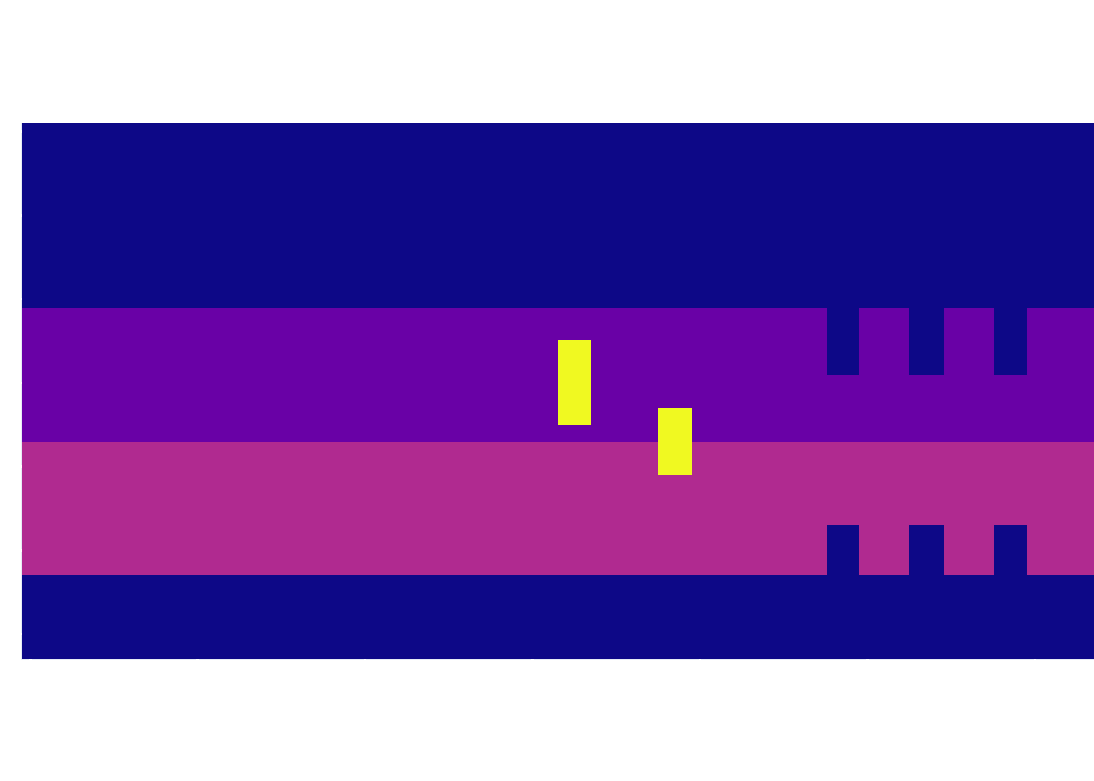
\includegraphics[scale=0.15]{images/agent_view.pdf}};
\draw[line width=0.046875cm, -latex] (5.250000, 0.35) -- (5.250000, 1.53);

%--------------------------------------------------------------------------------------------------------------------------------------------
% Policy Network
\draw[line width=0.046875cm, fill=ff_color, rounded corners=0.100000cm] (0.000000, 10.08) -- (2.500000, 10.08) -- (2.500000, 9.18) -- (0.000000, 9.18) -- cycle;
\node[text width=2.500000cm, align=center] at (1.250000, 9.68) {\footnotesize Policy \vspace{-0.3cm} \linebreak Network};

\node[text width=2.500000cm, align=center] at (0.312500, 11.580000) {$\pmb \mu$};
\node[text width=2.500000cm, align=center] at (1.250000, 11.580000) {$\pmb \sigma$};
\node[text width=2.500000cm, align=center] at (2.187500, 11.580000) {$ \hat V$};

\draw[-latex, line width=0.046875cm, rounded corners=0.200000cm] (1.250000, 10.730000) -- (0.312500, 10.730000) -- (0.312500, 11.33);
\draw[-latex, line width=0.046875cm, rounded corners=0.200000cm] (1.250000, 10.730000) -- (2.187500, 10.730000) -- (2.187500, 11.33);
\draw[line width=0.046875cm, -latex] (1.250000, 10.03) -- (1.250000, 11.33);

\draw[line width=0.046875cm, -latex] (1.250000, 6.230000) -- (1.250000, 9.23);
\draw[line width=0.046875cm, -latex] (4, 9.68) -- (2.5, 9.68);

\end{tikzpicture}
\caption[Multi-agent Transformer]{The Transformer model used in this thesis. On the right side, an ECA-ResNet processes visual input maps and outputs a vector representation. On the left side, the states of all agents $\Upsilon$ relative to the ego-agent are embedded and then fed into a Transformer encoder. The resulting $|\Upsilon|$ vectors are concatenated with the output of the convolutional pipeline. A parameter-shared \gls{mlp} policy decodes the concatenated representations, producing a distribution $(\pmb \mu, \pmb \sigma)$ and a value estimate $\hat V$ for each agent.}\label{fig:transformer}
\end{figure}
The architecture consists of two main components: First is a convolutional tower processing the visual map of the ego agent restricted to its own point of view. Note that all operations in the following description assume $3 \times 3$ kernels unless explicitly stated otherwise. After an initial convolutional layer, the image is downsampled using a pooling layer with stride $2$. This initial stage is followed by three basic convolutional blocks \cite{heDeepResidualLearning2015}, where the first convolution has stride $2$ and increases the number of filters by a factor of $2 \times$ over the output of the previous block. The second convolutional layer of each block uses stride $1$ and does not change the depth of the feature maps. All blocks use skip connections to alleviate the degradation problem \cite{heDeepResidualLearning2015}, which add the input of a block to its output. Before the block's input is added through the skip connection, an ECA-module learns global channel context \cite{wangECANetEfficientChannel2020}. Adding a channel-attention mechanism to the convolutional network is motivated by significant performance gains in applications to Go \cite{wuAcceleratingSelfPlayLearning2020}. The final component of the image processing pipeline consists of a fully convolutional head inspired by \cite{howardSearchingMobileNetV32019}. It uses two convolutional layers with $1 \times 1$ kernel size after applying an average pooling operation. The network output of the convolutional tower is a compact vector representation of the input image, denoted as $\mathbf m$.

The core component which lets the model learn interactions between a flexible number of agents is a Transformer encoder. The difference between the Transformer encoder and a decoder is that the encoder allows interactions in both directions of the sequence. The decoder on the other hand uses masking to ensure that only left-to-right dependencies are modeled\footnote{In natural language processing, this means that the encoder produces a bidirectional representation. BERT is a prominent example of such a model \cite{devlinBERTPretrainingDeep2019}. The decoder is instead used for classical language modeling, e.g. in the GPT architecture. Here the model cannot condition on future tokens, i.e. right to left dependencies \cite{devlinBERTPretrainingDeep2019}.}. Recall that an agent's numerical state $\mathbf s_i^{\text{num}} (t)$ consists of its own trajectory data as well as the relative trajectories of the other agents in the scenario (see Section~\ref{sssec:input_representation}). This can be interpreted as a sequence of objects between all of which interactions are learned by utilizing the multi-head attention mechanism. Following the steps outlined in Section~\ref{sssec:attention}, the agent trajectories are first normalized and then embedded using a single fully connected layer. This produces an $|\Upsilon| \times d_{model}$ representation matrix $\mathbf Z$, where $|\Upsilon|$ is the number of agents in the scenario. Then positional encodings are added, allowing the network to identify each agent in the sequence. In this work, learned positional embeddings are used compared to fixed sinusoidal ones \cite{devlinBERTPretrainingDeep2019}. The embedded and augmented agent trajectories are next fed into a Transformer encoder with four layers to learn bidirectional interactions between the agents. Finally, the output of the Transformer is a representation matrix $\mathbf T$ of size $|\Upsilon| \times d_{model}$.

To obtain a distribution for each agent in the scenario, each row of the matrix $\mathbf T$ is concatenated with the vector output $\mathbf m$ of the convolutional tower. This can be interpreted as a sequence of combined representations for each agent. The elements of the sequence are then fed into an \gls{mlp} policy network utilizing parameter-sharing. Reusing the network weights helps to keep the model as small as possible. In the final step, the policy outputs distribution parameters and value estimates for each agent.

The multi-agent Transformer architecture described in the previous paragraphs fulfills the requirement of being able to handle a flexible number of traffic participants. What is the intuition behind the model? Clearly an agent only receives information from its own sensors. Using itself as a model though, it can exploit the incomplete information obtained from other agents to approximate their action distributions. Of course this kind of modeling becomes coarser and coarser the further other agents are away. It is however not unlike humans make predictions about the immediate future of traffic situations. Drivers also have to plan using imperfect information, as they only perceive the road from their perspective.

The last part missing from the concept now that a network architecture has been determined is a training procedure. It is outlined in the next section.

\subsection{Training algorithm}\label{ssec:training_loop}
\begin{algorithm}[ht]
\SetAlgoLined
\begin{multicols}{2}
 Set Python, Numpy, PyTorch seeds to $S$.\\
 Initialize network parameters $\theta$ randomly.\\
 Initialize empty buffer $\mathcal D = \emptyset$.\\
 \For{$e=0$ \KwTo $E$}{
 \definecolor{shadecolor}{RGB}{0,128,0}
 \transparent{0.5}%
 \begin{shaded}
 {
 \transparent{1.0}%
 \While{$t < T$}{
    Load new network parameters $\theta$.\\
    Execute guided \gls{mcts}.\\
    Generate samples $(\mathbf s, \mathbf a, \mathbf n, \Vtarget) \sim \phat$.
  }
  }
 \end{shaded}
 \vspace{-1cm}
  \definecolor{shadecolor}{RGB}{0,0,139}
  \transparent{0.5}%
 \begin{shaded}
 {
 \transparent{1.0}%
  Store samples:\\ 
  $\mathcal D \leftarrow \mathcal D \cup \{ (\mathbf s, \mathbf a, \mathbf n, \Vtarget) \}_{t=1}^T$.\\
  \If{$|\mathcal D| > D$}{
    Remove $|\mathcal D| - D$ oldest samples.
   }
  \For{$p=0$ \KwTo $P$}{
    Draw $B$ samples $\{ (\mathbf s, \mathbf a, \mathbf n, \Vtarget) \}_{b=1}^B \sim \mathcal D$.\\
    Generate action log-probabilities $\log \pi_\theta (\mathbf a_b | \mathbf s_b)$.\\
    Generate value estimates $V_\theta (\mathbf s_b)$.\\
    Update $\theta \leftarrow \theta - \lambda \mathcal L_\theta (\mathbf a_b, \mathbf s_b)$.
  }
  }
   \end{shaded}
 }
 \columnbreak
 {
 \textbf{Algorithm components}\\
 Guided \gls{mcts} policy \phat \\
 Network policy \p\\
 Fixed size replay buffer $\mathcal D$\\ 
 ~\\
 }
 {
 \textbf{Hyperparameters}\\
 Seed $S$\\
 Replay buffer size $D$\\
 Number of Episodes $E$\\
 Number of samples $T$\\
 Number of training epochs $P$\\
 Batch size $B$\\
 Learning rate $\lambda$\\ 
 ~\\
 }
  {
 \textbf{Languages}\\
 \textcolor{cppgreen}{ \textbf{C++}}\\
 \textcolor{pyblue}{ \textbf{Python}}\\
  }
 \end{multicols}
 \caption{Guided \gls{mcts} training}
 \label{algo:training_algorithm}
\end{algorithm}
The high-level training procedure for the guided \gls{mcts} is described in Algorithm~\ref{algo:training_algorithm}. Before the first execution of the search, hyperparameters are loaded from a configuration file and used to set the seeds. Then an empty replay buffer $\mathcal D$ is constructed. The neural network parameters $\theta$ are initialized randomly at the start of the training. The algorithm then performs a data-collection and training loop for $E$ episodes.

During training, experiences are generated by executing the guided \gls{mcts} with the current network parameters $\theta$. At each stage of the search, the root node states $\mathbf s$, actions $\mathbf a$ and corresponding visitation counts $\mathbf n$ are exported\footnote{Subscripts $_0$ are omitted as only root node data is exported.}. Value targets $\Vtarget$ are obtained using Equation~\ref{eq:value_target} and saved as well. Note that the training data for all agents in the scenario is exported. This provides a regularization component by presenting the network with different ego perspectives for each scenario. More importantly, it speeds up data collection by a factor of $|\Upsilon| \times$, where $|\Upsilon|$ is the number of agents in a scenario. Since the generation of experiences is by far the most expensive computational component of the algorithm, training speed is improved significantly.

To further augment the training data, Gaussian noise is added to vehicle starting positions and scenario lane width. Given the noise standard deviations as $\sigma_{\text{lane}}, \sigma_{x}$ and $\sigma_{y}$ respectively, this results in:
\begin{align}
    w_{\text{lane}} & = \bar w_{\text{lane}} +  \epsilon_{\text{lane}}, & \epsilon_{\text{lane}}  &\sim \normal{0, \sigma_{\text{lane}}}\\
    x_i (0) & = \bar x_i (0) + \epsilon_x, & \epsilon_x & \sim \normal{0, \sigma_{x}} \\
    y_i (0) & = \bar y_i (0) + \epsilon_y, & \epsilon_y & \sim \normal{0, \sigma_{y}}~,
\end{align}
where $w_{\text{lane}}$ is the lane width and $(x_i (0), y_i (0) )$ is the starting position of agent $i$. The same quantities denoted with a bar correspond to the initial locations without noise.

Once the \gls{mcts} has generated $S$ samples, the data collection stops and all experiences are stored in the replay buffer $\mathcal D$. The buffer is using a fixed-size FIFO-queue, which is indicated in Algorithm~\ref{algo:training_algorithm} by the if-clause removing the oldest samples once the maximum size $D$ is reached. More sophisticated schemes of determining the buffer size exist, e.g. using a sublinear window function \cite{wuAcceleratingSelfPlayLearning2020} or an exponentially growing buffer \cite{anthonyThinkingFastSlow2017}. However, a fixed size queue keeps it simple and is sufficient to show the efficacy of the proposed approach.

After the generated experiences have been added to the dataset $\mathcal D$, a training loop iterates over the shuffled samples in the replay buffer $P$ times. First a batch of $B$ experiences is drawn from the buffer. The states $\mathbf s_b$ and actions $\mathbf a_b$ of the batch are used to generate action log-probabilities $\log \pi_\theta (\mathbf a_b | \mathbf s_b)$ and value estimates $V_\theta (\mathbf s_b)$ from the network. Criterion~\ref{eq:multi_agent_full} can now be evaluated by using the value targets $\hat V (\mathbf s_b)$ and visitation counts $\mathbf n_b$. The final part of a training step consists of performing a gradient descent update for the neural network parameters $\theta$.

Once the network training has concluded, a new episode $e$ is started with the updated parameters $\theta$. The training proceeds for a fixed number of steps. A high level description such as the one given above of course omits a number of implementation details. The next chapter therefore highlights the most crucial choices.





